\documentclass[../main.tex]{subfiles}

\graphicspath{{pictures/}{../pictures/}}

\chapterimage{chapter_head_2.pdf} % Chapter heading image

\begin{document}
	\chapter{Data Types}
	
	%----------------------------------------------------------------------------------------
	%	Basic Types
	%----------------------------------------------------------------------------------------
	
	\section{Basic Types}
	
	Much of programming is about the receiving, manipulating, and sending of data.  Since C is a typed language, it needs to know how to interpret the data that you are working with.  In many cases, the underlying bits that are actually being stored are the same.  However, based on the type assigned to that data, the C compiler will interpret it differently.  C can't really tell the difference between 41 and the letter 'A' (which has the ASCII value of 41).  Its up to you as the programmer to specify if the data is an integer or if its a character.
	
	Below are a few of the basic data types you'll encounter in C.	
	\begin{itemize}
		\item \textbf{int}		-	Represents whole numbers.
		\item \textbf{char}		-	Represents a single character.
		\item \textbf{float}	-	Represents numbers with decimal points (single precision).
		\item \textbf{double} 	-	Represents numbers with decimal points (double precision).
	\end{itemize}

	The platform that a program is compiled for can affect the number of bytes that a data type requires.  While most of today's platforms are 64-bit, there are still a few 32-bit systems out there.  If the max or min size of a data type is a concern to you, you'll want to be sure you know the size of that type on the platform your code will be compiled for.
	%----------------------------------------------------------------------------------------
	%	Integer
	%----------------------------------------------------------------------------------------	
	\subsection{Integers}
	
	By default, an \textit{int}\index{int} utilizes 4 bytes on both the 32-bit and 64-bit platforms. However, there are a couple of qualifiers that can affect how the data is interpreted as well as how many bytes are used.  
	\begin{itemize}
		\item \textbf{short}\index{short}	-	Utilizes 2 bytes (16 bits).
		\item \textbf{long}\index{long int}		-	Utilizes 4 bytes on a 32 bit platform and 8 bytes on a 64 bit platform.
		\item \textbf{long long}\index{long long int}-	Utilizes 8 bytes on a 32 bit platform and 8 bytes on a 64 bit platform.
		\item \textbf{signed}	-	Integers are \textit{signed} by default meaning they utilize two's complement to represent positive and negative numbers.  You do not need to specify \textit{signed} but can for greater clarity for someone reading your code.
		\item \textbf{unsigned}	-	As an \textit{unsigned} integer, there is no sign bit.  Therefore you can store larger positive numbers but you cannot store negative numbers.\\
	\end{itemize}
	
	\lstinputlisting[caption={\lstname}]{src/02-integer-32bit.c}
	
	\begin{lstlisting}[language=bash, numbers=none]
		$ file 02-integer-32bit
		02-integer-32bit: ELF 32-bit LSB shared object, Intel 80386
		
		$ ./02-integer-32bit 
		Number of Bytes:
		short int: 2
		int: 4
		long int: 4
		long long int: 8
		
		Value of signed   short: -275
		Value of unsigned short: 65261
		
		Min signed int: -2147483648
		Max signed int: 2147483647
		
		Min unsigned int: 0
		Max unsigned int: 4294967295
	\end{lstlisting}
	
	As you can see with the \textit{file} command, 02-integer-32bit has been compiled as a 32-bit binary.  Notice that an \textit{int} and \textit{long int} are both 4 bytes but a \textit{long long int} is 8 bytes.  
	
	Also notice on line 11 that I assign the value of -275 to \textit{si} which is a \textit{signed short int} and it prints out just fine on line 14.  However, when I print it out a second time on line 15 I cast it as an \textit{unsigned short int}.  Under the hood, the bits haven't changed; how they were interpreted did.  -275 is actually 1111111011101101 in binary.  The left-most bit (most significant bit) is the \textit{sign} bit.  When cast as an \textit{unsigned short int}, this bit is not longer interpreted as a signed bit which is why we now get a positive number.  I point this out only because it is important to note that you as the programmer need to understand the data you are working with because C only pays attention to whether or not you declared it as \textit{signed}\index{signed} or \textit{unsigned}\index{unsigned}.  To further demonstrate this, I've printed out the max and min value that a signed integer and an unsigned integer can hold.\\
	
	\lstinputlisting[caption={\lstname}]{src/02-integer-64bit.c}
	
	\begin{lstlisting}[language=bash, numbers=none]
	$ file 02-integer-64bit
	02-integer-64bit: ELF 64-bit LSB shared object, x86-64
	
	$ ./02-integer-64bit 
	Number of Bytes:
	short int: 2
	int: 4
	long int: 8
	long long int: 8
	\end{lstlisting}
	
	Notice this 02-integer-64bit is compiled as a 64-bit executable.  In this case, an \textit{int} is still 4 bytes but a \textit{long int} is now 8 bytes allowing you to store much larger numbers.  
	
	\subsubsection{stdint.h}
	
	The \textit{stdint.h} header imports other header files such as \textit{stdint-intn.h} and \textit{stdint-uintn.h} that specify a number of macros and type definitions (\textit{typedef}) to make working with integers more consistent across 32-bit and 64-bit platforms.  By using it, you can guarantee the size of the resulting integer. 
	\begin{itemize}
		\item \textbf{uint8\_t}, \textbf{uint16\_t}, \textbf{uint32\_t}, \textbf{uint64\_t} - All unsigned integers that utilize 8-bit, 16-bit, 32-bit, and 64-bit accordingly.
		\item \textbf{int8\_t}, \textbf{int16\_t}, \textbf{int32\_t}, \textbf{int64\_t} - All signed integers that utilize 8-bit, 16-bit, 32-bit, and 64-bit accordingly.
	\end{itemize}

	Due to the inconsistent sizes for integers we identified between 32-bit and 64-bit platforms, you'll often see code that uses the \textit{stdint.h} header file and specifies the actual size that is needed.  
	
	Additionally, \textit{stdint.h} also specifies macros for the MAX and MIN sizes of various integers.  You may decide to use these in your programs to test for an overflow of an integer.
	
	\begin{verbatim}
	/* Minimum of signed integral types.  */
	# define INT8_MIN               (-128)
	# define INT16_MIN              (-32767-1)
	# define INT32_MIN              (-2147483647-1)
	# define INT64_MIN              (-__INT64_C(9223372036854775807)-1)
	/* Maximum of signed integral types.  */
	# define INT8_MAX               (127)
	# define INT16_MAX              (32767)
	# define INT32_MAX              (2147483647)
	# define INT64_MAX              (__INT64_C(9223372036854775807))
	
	/* Maximum of unsigned integral types.  */
	# define UINT8_MAX              (255)
	# define UINT16_MAX             (65535)
	# define UINT32_MAX             (4294967295U)
	# define UINT64_MAX             (__UINT64_C(18446744073709551615))
	\end{verbatim}
	
	\subsubsection{stddef.h}\index{size\_t}
	This header file defines a number of additional types as well as macros.  
	
	One type that you will see quite frequently is \textit{size\_t}.  This is an \textit{unsigned integer} that is often returned when the result is the number of bytes of something.  For example, the manpage for \textit{strlen} function shows:
	
	\begin{verbatim}
	SYNOPSIS
	#include <string.h>
	
	size_t strlen(const char *s);
	
	DESCRIPTION
	The strlen() function calculates the length of the string pointed to by s, 
	excluding the terminating null byte ('\0').
	
	RETURN VALUE
	The strlen() function returns the number of bytes in the string pointed to 
	by s.
	\end{verbatim}
	
	So the \textit{strlen} function returns the number of bytes in the string as type \textit{size\_t} which under the hood, is really just an \textit{unsigned int}.
	
	\subsubsection{stdbool.h}\index{bool}
	Languages other than C, often have a type for boolean variables.  These are variables that can only hold the value of \textit{true} or \textit{false}.  C accomplishes this with a set of macros which under the hood are really just integer constants.
	
	\begin{itemize}
		\item \textbf{true} - constant 1
		\item \textbf{false} - constant 0
	\end{itemize}

	You may see these returned from functions to indicate whether something was successful or not.  As a programmer using type \textit{bool} as a return may make it easy to ascertain the reason behind what a function is returning.  However, be cautious about using them to test the return from standard library functions.  In many cases, a success is returned as a zero but a failure is returned as a non-zero number.  It is always a good idea to read the manual page of a function to understand what it uses for return types and what the return values actually mean. 
	
	%----------------------------------------------------------------------------------------
	%	Characters
	%----------------------------------------------------------------------------------------

	\subsection{Characters}
	
	A \textit{char}\index{char} within C typically requires just a single byte to store a single character.  This is based upon the fact that the \textit{char} was meant to store the ASCII\index{ASCII} value which only required 7 bits.  Depending upon the type of project you are working on, this may or may not be sufficient. Below is the ASCII chart \ref{fig:ascii} as printed out by running the \textit{ascii} command on the terminal.  Notice the values only go upto 127.
	
	\begin{figure}[h]
		\centering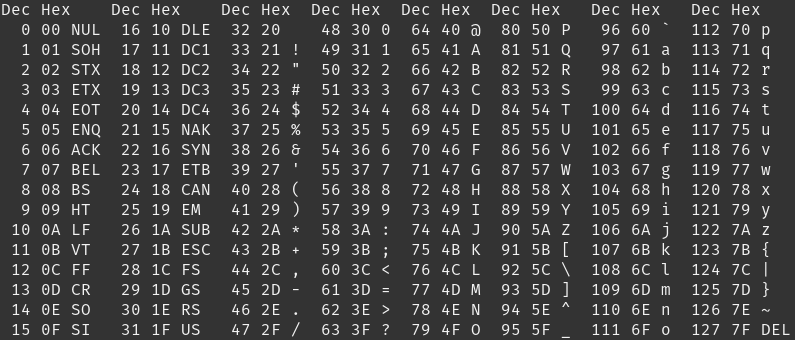
\includegraphics[scale=0.5]{ascii.png}
		\caption{ASCII Chart}
		\label{fig:ascii} % Unique label used for referencing the figure in-text
	\end{figure}
	
	Obviously the ASCII chart was built for the English language.  When not sufficient, there are ways of using an \textit{unsigned int} and \textit{UTF-8} encoding instead.  Additionally, there are wider character data types such as \textit{wchar\_t} that utilize more than 1 byte in order to store character values by their Unicode value rather than an ASCII value.  I will not be going into these methods and alternate data types but if it interests you, I suggest checking out articles such as \href{https://www.cprogramming.com/tutorial/unicode.html}{https://www.cprogramming.com/tutorial/unicode.html}.\\
	
	\lstinputlisting[caption={\lstname}, label={lst:ternary_conditional_evaluation}]{src/02-character1.c}
	
	\textbf{Line 2}: Here I import \textit{ctype.h}.  Doing so gives me access to a number of functions and macros pertaining to the use of characters.\\
	\textbf{Line 7}: Here I declare a \textit{char} and give it the value of \textit{a}.  Notice it holds a single character and I use single quotes.\\
	\textbf{Line 8}: Here I use the function toupper which has a function \textit{declaration} of \textbf{int toupper(int c);}.  This is our first indication that under the hood, a \textit{char} is treated very much like an \textit{int}.\\
	\textbf{Line 14}: Here I use the function \textit{isalpha} to test to see if the character is alphabetic.\\
	\textbf{Line 22}: Here I use the function \textit{isdigit} to test to see if the character is a digit.\\
	
	By typing '\texttt{man 3 toupper}' on the terminal, I am presented with the manual page describing the C \textit{toupper} function:\\
	
	\begin{figure}[h]
		\centering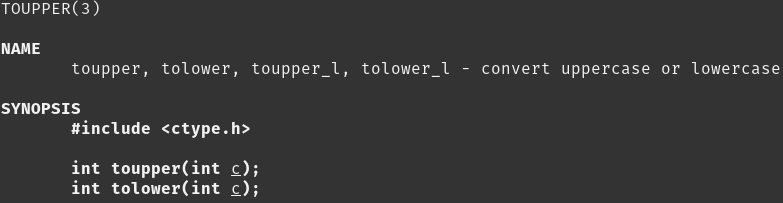
\includegraphics[scale=0.5]{toupper.png}
		\caption{toupper}
		\label{fig:toupper} % Unique label used for referencing the figure in-text
	\end{figure}

	Likewise, I can view the manpage for \textit{isdigit} by typing '\texttt{man 3 isdigit}'.\\
	
	\begin{figure}[h]
		\centering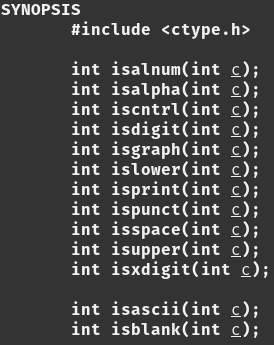
\includegraphics[scale=0.5]{isalpha.png}
		\caption{isalpha, isdigit}
		\label{fig:isapha} % Unique label used for referencing the figure in-text
	\end{figure}

	\subsubsection{Character Constants}\index{character constant}
	
	A character constant is any character surrounded by single quotes.  For example, when we assigned 'a' to \textit{c1} in the previous example, that was an example of a character constant.  However, if we were using wider characters other than the standard \textit{char}, we may want to pass in the Unicode value.  To do this we may specify \textit{u'$\textbackslash$x3b3'}\cite{c_nutshell}.    
	
	The \textit{\textbackslash} we just saw with \textit{$\textbackslash$x} known as an escape sequence.  There are a number of other escape sequences you may encounter.  You've already seen me use '\textit{$\textbackslash$n}' int nearly every \textit{printf}.  This is a character constant for the newline character.  Some of the other character constants you may encounter are:
	\begin{itemize}
		\item \textbf{$\textbackslash$0}	- The NULL character.  You'll often see this as terminating a character array.
		\item \textbf{$\textbackslash$n}	- New line.
		\item \textbf{$\textbackslash$r}	- Carriage return.
		\item \textbf{$\textbackslash$t} 	- Horizontal tab.
		\item \textbf{$\textbackslash$v}	- Vertical tab.
		\item \textbf{$\textbackslash$o}	- Octal values.  This will look something like \textit{$\textbackslash$o456} where we are referring to octal value 456 which is 302 in decimal.
		\item \textbf{$\textbackslash$x}	- Hexidecimal values.  This will look something like \textit{$\textbackslash$x456} where we are referring to hexadecimal 456 which is 1110 in decimal.
		\item \textbf{$\textbackslash$u}	- Unicode values.	
	\end{itemize}

	%----------------------------------------------------------------------------------------
	%	Floats
	%----------------------------------------------------------------------------------------
	
	\subsection{Floats}
	
	Floating point numbers are numbers with decimal points.  Just as with integers, the data type affects the number of bytes used to store values.  With integers, concern was with max and min values as well as overflows.  With floats, its about precision.  A floating point value is an approximation and the cost of being more precise in that approximation is in the number of bytes that are required to store it.
	
	Below is a chart directly taken from the book "C in a Nutshell"\cite{c_nutshell}.
	\begin{table}[h]
		\centering
		\begin{tabular}{l l l l l}
			\toprule
			\textbf{Type} & \textbf{Storage Size} & \textbf{Value Range} & \textbf{Smallest positive Value} & \textbf{Precision}\\
			\midrule
			float\index{float} & 4 bytes & $\pm$3.4$\epsilon$+38 & 1.2$\epsilon$-38 & 6 digits \\
			double\index{double} & 8 bytes & $\pm$1.7$\epsilon$+308 & 2.3$\epsilon$-308 & 15 digits \\
			long double\index{long double} & 10 bytes & $\pm$1.1$\epsilon$+4932 & 3.4$\epsilon$-4932 & 19 digits \\
			\bottomrule
		\end{tabular}
		\caption{Real floating-point types}
		\label{tab:floating-point} % Unique label used for referencing the table in-text
	\end{table}

	\lstinputlisting[caption={\lstname}]{src/02-float1.c}
	
	\begin{lstlisting}[language=bash, numbers=none]
		$ ./02-float1 
		1 / 3 = 0.000000
		1 / 3 = 0.333333
	\end{lstlisting}
	
	\textbf{Line 7}: On this line, 1 is divided by 3 and the results are stored in \textit{x}.  However, when \textit{x} is printed out on line 8, we see that what actually got stored is 0.0.  This is because we divided one integer by another integer.  In C, this will result in another integer.  Since integers cannot have decimal points, 0 gets stored in X.\\
	\textbf{Line 10}: Again we do the same division but instead of dividing two integers, we first cast 1 as a \textit{float}.  Under the hood, this operation should result in a \textit{double} being generated but because we are storing it in a \textit{floatmathmatical}, it it rounded to 6 digits of precision.  We can see this when we print \textit{x} on line 11 in that there are only 6 digits (leading and trailing zeros are ignored).
	
	There is another header file called \textit{complex.h} that allows for the use of complex floating point types.  I will not be discussing them here.
	
	%----------------------------------------------------------------------------------------
	%	Enum
	%----------------------------------------------------------------------------------------
	\section{Enum}
	An \textit{enum}\index{enum} is a data type that consists of named values that correspond to integer constants. Often times it makes sense to use an \textit{enum} rather than to constant to make it ee In the previous chapter, we built an enum in our header file to represent Mystery Inc members.
	
	\lstinputlisting[caption={\lstname}]{src/01-helper.h}
	
	By default, FRED would correspond to the value of 0, DAPHNE to 1, VELMA TO 2, SHAGGY to 3, and SCOOBY to 4.  However, I could have specified different values.
	
	\begin{verbatim}
	enum temperature {
	    FAHRENHEIT = 1,
	    CELCIUS = 2,
	}
	\end{verbatim}
	
	Depending upon the coding standard you are following, it is often customary to pair up an \textit{enum} definition with a type declaration \textit{typedef}\cite{embedded_c}\index{typedef} and to name the resulting type with a trailing "\_t" to signify it is a custom type.  
	
	\section{Void}
	In chapter 1, I mentioned a function can indicate it returns no values by using the \textit{void}\index{void} keyword.  However, \textit{void} can be a type as well.  C uses them with pointers all the time.  We'll discuss pointers shortly but for now, a \textit{void} pointer holds a memory address but does not indicate the data type that resides at the address.  This can be useful in making certain types of functions or data types generic to the data that they store or manipulate at the cost of additional code complexity.
	
	\clearpage
	%----------------------------------------------------------------------------------------
	%	Operators
	%----------------------------------------------------------------------------------------	
	\section{Operators}
	
	The following operators are some of the most common you'll see when writing C.  I won't go into depth with them as you'll see most of them used in further examples.
	
	\begin{table}[h]
		\centering
		\begin{tabular}{l l l}
			\toprule
			\textbf{Operator} & \textbf{Purpose} & \textbf{example}\\
			\midrule
			* 	& Multiplication 	& a * b \\
			/ 	& Division 			& a / b \\
			+ 	& Addition 			& a + b \\
			- 	& Subtraction 		& a - b \\
			\% 	& Modulus (remainder) & a \% b \\
			++ 	& Increment 		& ++a or a++ \\
			\verb|--| & Decrement 	& \verb|--|a or a\verb|--| \\
			\& 	& BITWISE AND 		& a \& b \\
			| 	& BITWISE OR 		& a | b \\
			\textasciicircum 	& BITWISE XOR 		& a \textasciicircum b \\
			\textasciitilde 	& BITWISE NOT 		& $\textasciitilde$a \\
			<< 	& Left Shift 		& a << 2 \\
			>> 	& Right Shift 		& a >> 2 \\
			= 	& Assignment 		& c = a + b \\
			==	& Equality 			& a == b \\
			<	& Less than			& a < b \\
			>	& Greater than		& a > b \\
			<=	& Less than or equal to & a <= b \\
			>=	& Greater than or equal to & a >= b \\
			!	& Negation (NOT)	& !a \\
			\&\&& Logical AND		& a \&\& b \\
			|| 	& Logical OR		& a || b \\
			\&	& Address of		& \&a \\
			*	& Indirection		& *a \\
			{[ ]}	& Subscript		& a[b] \\
			.	& Struct or Union member designator & a.b \\
			->	& Struct or Union member designator by Reference & a->b \\
			sizeof & Storage size of object & sizeof(a) \\
			?:	& Conditional Evaluation & a ? b : c \\
			\bottomrule
		\end{tabular}
		\caption{Operators}
		\label{tab:operators}
	\end{table}

	The Assignment '=' operator is often combined with other operators such as '+', '-', '/', ' to shorten the amount of code the programmer has to type.  For example, \texttt{a += 5} is equivalent to \texttt{a = a + 5}.
	
	Just as in mathematical equations, certain operations are given precedence over other operations.  The same is true for C, certain operators have precedence\index{operator precedence} over other operators. "C in a Nutshell"\cite{c_nutshell} has a good chart listing them out in Chapter 5.  A small sampling of the chart shows that the postfix operators such as \texttt{[ ]}, \texttt{.}, and \texttt{->} have precedence over the unary operators \texttt{*}, \texttt{\&}, \texttt{!}, and \texttt{\textasciitilde} which have precedence over multiplication operators \texttt{*}, \texttt{/}, and \texttt{\%}.  This list goes on an on for the remainder of the operators.  It is good to generally understand the precedence but I don't suggest you rely on them.  Instead, I suggest taking following the guidance given in the "Embedded C Coding Standard"\cite{embedded_c}:

	\begin{quotation}
		a.	Do not rely on C's operator precedence rules, as they may not be obvious to those who maintain the code.  To aid clarity, use parentheses (and / or break long statements into multiple lines of code) to ensure proper execution order within a sequence of operations.\\
		b.	Unless it is a single identifier or constant, each operand of the logical AND (\&\&) and logical OR (||) operators shall be surrounded by parentheses.
	\end{quotation}
	
	Lets take a look at an example that uses a few of these operators.  Don't worry if it doesn't all make sense yet.\\
	
	\lstinputlisting[caption={\lstname}, label={lst:xor}]{src/02-xor.c}
	
	\textbf{Line 11}: Here we assign a string constant to a \textit{char} array.  We utilize the subscript operators \texttt{[ ]} to designate that the variable \textit{clear} is a \textit{char} array.  We'll talk about \textit{arrays} in future sections.  We also use the assignment operator \texttt{=} to assign the address of the string constant to the \textit{char} array.\\
	\textbf{line 13}: We run the function \textit{stringlen} to get the length of the string stored in the \textit{character array} and use the assignment operator \texttt{=} to store the result in \textit{keyLen}.\\
	\textbf{Line 35}: \textit{Original} and \textit{key} are pointers\index{pointer} (which we haven't discussed thus far).  We know this because the arguments use the indirection operator \texttt{*}.  Pointers hold addresses so when we use the indirection operator, what we are getting back is the thing that the pointer points to.  In this case, they should point to the first character of the string constants that got assigned to \textit{clear} and \textit{key} from earlier.  However, reaching into a pointer without first checking to make sure they actually hold an address is dangerous.  This is why we use the equality operator \texttt{==} to see if they point to \textit{NULL}\index{NULL}; a macro set to 0.  In other words, if our program has been handling pointers correctly up to this point, they should contain either a valid address or 0.  By testing for \textit{NULL} at the beginning of our function, we can be assured that moving forward, the pointers actually point to something.\\
	\textbf{Line 40}: This may be our first example utilizing a \textit{for} loop.  Don't worry, we'll talk about control flow in coming sections.  For now, we use the assignment control operator \texttt{=} to set an initial value for variable \textit{i}.  We also utilize the less than operator \texttt{<} to make sure the value of \textit{i} doesn't exceed the value of \textit{oLen}.  This would indicate we've passed the end of the \textit{char} array.  Additionally we use the increment operator \texttt{++} to increment the value of \textit{i} after each loop.\\
	\textbf{Line 41}:  In this line we use the subscript operators \texttt{[ ]} to operate on a single \textit{char} within the \textit{char} array.  In this case, \textit{i} is an index value that starts at 0 (corresponding to the first character in the \textit{char} array) and by incrementing by 1 after each loop, we'll XOR against each character.  We then combine the XOR operator \texttt{\textasciicircum} with the assignment operator \texttt{=} to form \texttt{$\textasciicircum$=}.  This means that we will XOR\index{XOR} the \textit{char} on the left side with the \textit{char} on the right side of this operator, and assign the result back to the same location as the original \textit{char} on the left. So what character are we using on the right?  Here we use the subscript operators \texttt{[ ]} once again to pull out a single \textit{char} from \textit{key}.  We utilize the modulus operator \texttt{\%} with index \textit{i} and \textit{kLen} which is the length of the key.  Since a modulus does remainder division, what we essentially get is a number between 0 and kLen - 1.  This allows us to loop back over each character within \textit{key} until we've gone all the way through each character in \textit{original}.  
	
	%----------------------------------------------------------------------------------------
	%	Arrays
	%----------------------------------------------------------------------------------------	
	
	\section{Arrays}\index{array}
	
	Arrays are objects that can contain multiple elements of the same type.  All elements are stored in a contiguous block of memory.  The number of elements is determined when the array is created and cannot be adjusted during its lifetime.  Individual elements of the array can be accessed via an index value that starts at 0.  This is why in the previous example, we started \texttt{i} with a value of 0 so that it would start at the beginning of the \textit{char} array.  

	Most arrays sizes are determined by the programmer at compile time by passing in integer constants.  You can however, have variable sized arrays.  I tend not to use these and have compiler flags that will complain if the size of an array can't be determined at compile time because it is the result of an expression or user input.  Instead I would use dynamic memory by building my array on the heap.  We'll discuss dynamic memory in a later section.
	
	In the XOR example we saw earlier, we saw a \textit{char} array for \textit{clear} and \textit{key}.  Those were single dimension arrays.  However, you can add additional dimensions by adding additional subscript operators \texttt{[ ]}.
	
	It is almost a good idea to initialize a variable with a value.  This is especially true for arrays since not every element may be used right away.  When the memory is allocated for the array, whatever happens to be at the memory address will show up in the array.  This can cause problems down the road as you have no way of knowing how that value arrived.  For example:\\
	
	\lstinputlisting[caption={\lstname}]{src/02-array1.c}
	
	\textbf{Line 9}: Here I hardcode the size of the array through the use of a \textit{\#define}\index{\#define} macro.  Doing this makes it obvious what the dimensions of the array are for but won't trigger the compiler into thinking I'm creating a variable sized array. The use of \textit{\#define} should be used in very limited cases\cite{embedded_c}.\\
	\textbf{Line 9}: A two-dimensional array is created to track students and their grades.  All of the grades will be of type \text{float}. Notice that this creates space for the array but does not assign it any values.\\
	\textbf{Line 10}: The \text{sizeof}\index{sizeof} operator determines how many bytes were allocated for the array.\\
	\textbf{Line 15}: This line runs inside of a nested for loop where the inner loop increments the \textit{test} index and the outer loop increments the \textit{student} index.  The end result is that we get all the grades for the first student and then each of the grades for each remaining student.\\
	
	\begin{lstlisting}[language=bash, numbers=none]
		$ ./02-array1 
		Grades consumes 24 bytes of memory.
		Student 0	Test: 0	Grade: 0.000000
		Student 0	Test: 1	Grade: 0.000000
		Student 0	Test: 2	Grade: 0.000000
		Student 1	Test: 0	Grade: 0.000000
		Student 1	Test: 1	Grade: 1158749014972294498713827247390720.000000
		Student 1	Test: 2	Grade: 0.000000
	\end{lstlisting}
	
	Notice because I didn't initialize the contents of the array, I pick up a stray value that happened to already be in memory when the array space was allocated there.\\
	
	\lstinputlisting[caption={\lstname}]{src/02-array2.c}
	
	\textbf{Line 10}:  I now initialize my \textit{grades} array by placing a zero in curly braces.  This zeros out each of the grades.\\
	\textbf{Line 9}: Here I under-allocate the size of the strings which are nothing more than \textit{char} arrays.  This causes no compile time warnings or errors.  However, as you'll see in the following output, this causes an issue in printing the first name in the array. The way that C knows it has reached the end of a string is that it reaches a null termination \texttt{$\textbackslash$0}\index{null terminator} character.  Since I under-allocated for the array, the first \textit{char} if the next string overwrites the \texttt{$\textbackslash$0}.  This is why they print out together when trying to print just the first string.  Just as disturbing and potentially distructive is the final \texttt{$\textbackslash$0} for the last name technically writes into memory that is not allocated to the \textit{students} array.\\


	\begin{lstlisting}[language=bash, numbers=none]
		$ ./02-array2 
		Grades consumes 24 bytes of memory.
		Student JennyJimmy	Test: 0	Grade: 0.000000
		Student JennyJimmy	Test: 1	Grade: 0.000000
		Student JennyJimmy	Test: 2	Grade: 0.000000
		Student Jimmy	Test: 0	Grade: 0.000000
		Student Jimmy	Test: 1	Grade: 0.000000
		Student Jimmy	Test: 2	Grade: 0.000000
	\end{lstlisting}
	
	%----------------------------------------------------------------------------------------
	%	Pointers
	%----------------------------------------------------------------------------------------
	
	\section{Pointers}\index{pointer}
	
	Pointers are used frequently in C so being proficient in their use is a must.  We've seen previously in the XOR example that pointers do as their name suggests; they point to things.  They contain the memory addresses.  Passing around memory address rather than entire objects is often times much more efficient than moving and copying values.  However, misuse of pointers can lead to buggy and insecure programs.  A common theme you may see is the \textbf{ABC} principle\index{ABC principle}.  \textbf{A}lways \textbf{B}e \textbf{C}hecking.  In otherwords, its good practice to always test your pointers before reaching into them.  I believe I mentioned this already but its worth repeating.  Reaching into a pointer that is set to \textit{NULL}\index{NULL} will cause a \textit{Segmentation fault} and cause your program to terminate.
	
	You'll often use the \textit{\&} operator when you need the memory address of something in order to pass it to a pointer.  You will also see the dereference \textit{*} operator used on a pointer to work with the data that resides at the memory address of the pointer.  In other words, the data that the pointer points to.  Using subscript operators \texttt{[ ]} with pointers is also quite common.  This can be used to dereference into a portion of the memory address based on index value and the data type of the pointer.  For example, lets assume we have a integer pointer and on a particular platform, an \textit{int} uses 4 bytes.  If we dereference into the 5th index position, we're going 20 bytes (4 * 5) passed the address held by the pointer.  In the following example, we'll see an example of this using a non-optimized version of a sorting algorithm.\\
	
	\lstinputlisting[caption={\lstname}, label={lst:pointers}]{src/02-pointers1.c}
	
	\begin{lstlisting}[language=bash, numbers=none]
		$ ./02-pointers1 
		1 9 7 15 42 18 12  
		1 7 9 12 15 18 42
	\end{lstlisting}
	
	\textbf{Line 15}: An array is declared to hold various integer values. The size of the array is based on the number of elements I initialize it with.\\
	\textbf{Line 17}: We calculate the number of elements in the array.  This works fine with arrays but as soon as I pass it to the \textit{sort} function and it becomes a pointer, it no longer works\cite{embedded_c}.  Instead, if I use the \textit{sizeof} on a pointer, what I'll get is the number of bytes required to store the address.  This will equate to 4 bytes on a 32 bit system and 8 bytes on a 64 bit system.\\
	\textbf{Line 21}: We pass the \textit{numbers} array to our \textit{sort} function.  I don't have to use the \texttt{\&} operator since \textit{numbers} being an array can automatically be interpreted in the called function as an \textit{int *} (integer pointer).  We also pass in the number of elements in our array since the \textit{sort} function will not be able to determine this.\\
	\textbf{Line 29}: We receive the \textit{numbers} array address as \textit{int *pArray}.  I have the option to name it anything I want.  Depending upon the coding standard you are following, often times giving the pointer a name that also indicates its a pointer can help in the readabilily later on\cite{embedded_c}. In this case, by starting the name with a 'p' its more obvious that its a pointer.\\
	\textbf{Line 30}: We check to make sure we received an address and not a \textit{NULL} pointer. This is something you must do each time you are about to use a pointer.  Not doing this is asking for your program to crash.\\
	\textbf{Line 38}: The subscript operators \texttt{[ ]} can still be used to access values within the array.\\
	\textbf{Line 40}: This line passes two different pointer addresses to our \textit{swap} function using pointer arithmetic.  Under the hood, the pointer \textit{pArray} is an integer pointer.  An \textit{int} takes up 4 bytes so what we're actually doing is \textit{ADDRESS + (i * 4)} to calculate the adjusted address that we actually send to the \textit{swap} function.  This is the exact same math that gets applied when we use the subscript operators \texttt{[ ]}.  However, I didn't want to dereference into the array and access the value at a particular address.  I wanted the address itself.  I could have also used \texttt{\&pArray[i]} and gotten the same results. Care must be taken as C won't stop you from calculating addresses passed the original array address space.\\
	\textbf{Line 48}: I once again check to ensure I received pointers that contain addresses and not \textit{NULL}.\\
	\textbf{Lines 53 - 55}: Here we move the values between the pointers by defreferencing them via the \texttt{*} operator.  In essence, we copy the value at the memory address pointed to by \textit{p1} into temp.  We then copy the value at the memory address pointed to by \textit{p2} into the memory address pointed to by \textit{p1}.  Finally, we copy the value of temp into the memory address pointed to by \textit{p2}.\\
	
	%----------------------------------------------------------------------------------------
	%	Dynamic Memory
	%----------------------------------------------------------------------------------------
	
	\section{Dynamic Memory}
	
	
	
	\subsection{Stack}
	Up until this point, the variables we've created have a lifetime based on the control block they were created in.  For example, in \textit{src/01-helper.c} (\ref{lst:distributeSnacks}), the \textit{num} variable is created at the top of the \textit{distributeSnacks} function and is automatically cleaned up at the closing bracket of the function.  Lets take a look at the \textit{01-basics3} program we looked at in chapter 1.  In order to produce the below code, I decompiled the executable by running: \texttt{objdump -M "intel" -d 01-basics3}. Below is a copy of the decompiled \textit{main} and \textit{distributeSnacks} functions. \\ 
	
	\begin{lstlisting}[language={[x86masm]Assembler}]
	0000000000001149 <main>:
	1149:	f3 0f 1e fa          	endbr64 
	114d:	55                   	push   rbp
	114e:	48 89 e5             	mov    rbp,rsp
	1151:	48 83 ec 10          	sub    rsp,0x10
	1155:	c7 45 fc 03 00 00 00 	mov    DWORD PTR [rbp-0x4],0x3
	115c:	8b 45 fc             	mov    eax,DWORD PTR [rbp-0x4]
	115f:	89 c7                	mov    edi,eax
	1161:	e8 1a 00 00 00       	call   1180 <distributeSnacks>
	1166:	89 c6                	mov    esi,eax
	1168:	48 8d 3d 95 0e 00 00 	lea    rdi,[rip+0xe95]
	116f:	b8 00 00 00 00       	mov    eax,0x0
	1174:	e8 d7 fe ff ff       	call   1050 <printf@plt>
	1179:	b8 00 00 00 00       	mov    eax,0x0
	117e:	c9                   	leave  
	117f:	c3                   	ret 
	
	0000000000001180 <distributeSnacks>:
	1180:	f3 0f 1e fa          	endbr64 
	1184:	55                   	push   rbp
	1185:	48 89 e5             	mov    rbp,rsp
	1188:	89 7d ec             	mov    DWORD PTR [rbp-0x14],edi
	118b:	c7 45 fc 00 00 00 00 	mov    DWORD PTR [rbp-0x4],0x0
	1192:	83 7d ec 03          	cmp    DWORD PTR [rbp-0x14],0x3
	1196:	74 08                	je     11a0 <distributeSnacks+0x20>
	1198:	83 7d ec 04          	cmp    DWORD PTR [rbp-0x14],0x4
	119c:	74 0b                	je     11a9 <distributeSnacks+0x29>
	119e:	eb 12                	jmp    11b2 <distributeSnacks+0x32>
	11a0:	c7 45 fc 14 00 00 00 	mov    DWORD PTR [rbp-0x4],0x14
	11a7:	eb 10                	jmp    11b9 <distributeSnacks+0x39>
	11a9:	c7 45 fc 28 00 00 00 	mov    DWORD PTR [rbp-0x4],0x28
	11b0:	eb 07                	jmp    11b9 <distributeSnacks+0x39>
	11b2:	c7 45 fc 00 00 00 00 	mov    DWORD PTR [rbp-0x4],0x0
	11b9:	8b 45 fc             	mov    eax,DWORD PTR [rbp-0x4]
	11bc:	5d                   	pop    rbp
	11bd:	c3                   	ret    
	11be:	66 90                	xchg   ax,ax
	\end{lstlisting}
	
	If you've never looked at assembly code before, this can look a bit crazy.  Without going into the nitty gritty details of assembly\index{assembly} language syntax, I wanted to take a second and point out a few things.  There is something called a \textbf{stack frame}\index{stack frame}.  \textit{Stack frames} typically hold the variables declared during compilation time.  What do I mean about during compilation time?  Essentially, the compiler has enough information during compilation to determine how much space to allocate for a variable and what its lifetime will be.  Each function gets its own stack frame.  This is somethine worth considering especially for recursive functions (functions that call themselves) because for each call, a new stack is provisioned.  There is also something called a \textbf{call stack}\index{call stack} that is composed of various stack frames and the return addresses associated with them.  This is demonstrated in figure \ref{fig:callstack}.
	
	\begin{figure}[h]
		\centering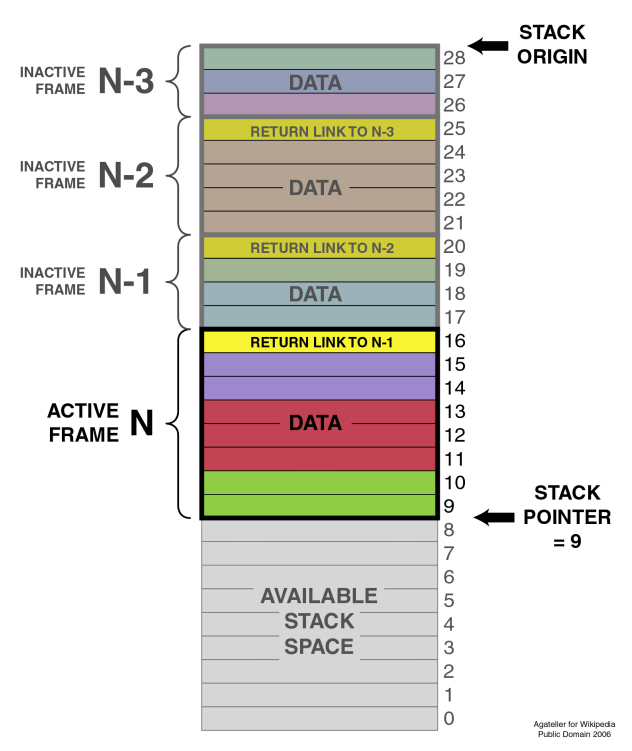
\includegraphics[scale=0.3]{callstack.png}
		\caption{Call Stack}
		\label{fig:callstack}
	\end{figure}

	In essence, as one function calls another, a new \textit{stack frame} is built so that the called function has a place to store its variables and the program knows where to go back to once that called function is complete.  There are two registers within the processor that keep track of the start and end of the \textit{stack frame}.  The \textbf{rbp}\index{rbp} (base pointer)  register marks the bottom and the \textbf{rsp}\index{rsp} (stack pointer) register marks the top of the stack frame.  In the context of the assembly code above, you can see on lines 3-5, the main function is establishing its stack by saving the address of the current base pointer (\textit{push rbp}), establishing a new location for the new base pointer (\textit{mov rbp, rsp}), and then subtracting 16 bytes (\textit{sub rsp, 0x10}) from the stack pointer (\textit{rsp}) to establish 16 bytes worth of space on the new stack for storing variables.  Again, you don't need to understand assembly code but I wanted you to see this in action in order for you to understand the purpose of the stack.  Of note, notice that we subtract in order to allocate space.  This means that the stack actually grows down in memory addresses.  We can then see on line 7 that the value 3 is being copied onto the stack at location \textit{rbp - 0x4}.  This correlates to where we created the variable \textit{member} and assigned to it the value of \textit{SHAGGY} back in \textit{01-basics3.c}(\ref{lst:basics3}).
	
	On line 9, we also see a \textit{call} to the \textit{distributeSnacks} function.  There is another register that keeps track of the current line or instruction that is being executed (\textbf{rip}\index{rip} - instruction pointer).  The \textit{call} first pushes \textit{rip + 1} onto the stack. This is so that when we return from \textit{distributeStacks}, execution will resume on line 10.  Then \textit{rip} is set to begin executing at the beginning of the \textit{distributeSnacks} function.  The \textit{return} on line 36 performs a \textit{pop rip} which pulls the return address off of the stack and places it in \textit{rip}.  This is why execution returns to line 10.
	
	For whatever reason, when the gcc compiler built this program, it didn't create a new stack for function \textit{distributeSnacks} large enough to store the \textit{num} variable.  This could be because the program is so small and this was a small optimization that the compiler made.  Whatever the reason, we can see that on lines 20 and 21, we save the address of our current base pointer address by pushing it on the stack and then set it equal to the current stack pointer address.  Although this is a whole new stack frame, it doesn't allocate space to save any variables by subtracting from the stack pointer.  Instead, we can see that on line 23, its actually storing its values in the previous stack frame.  Again, this is probably an optimization that saves one or two CPU cycles.
	
	Moving things on and off the stack is very common and fairly quick.  However, there are advantages and disadvantages for doing so.  One disadvantage is that because the return addresses for the calling function lives on the stack, its a place that a malicious user may want to attack in order to control what the program does upon returning from the called function.  A lot of work has been put into protecting the stack and detecting \textit{stack smashing} but nothing is full proof.  Additionally, because a \textit{stack frame} gets torn down after a function returns, the variables that lived there are no longer reachable.  Normally this is the functionality that you want but not always.  Instead, you may have reasons for wanting to allocate a larger amount of memory away from the rest of your stack variables or maybe you want it to outlive the end of the called function.  Additionally, you may not know how much memory you're going to require at the time of compilation.  Therefore, the compiler won't know how much space to allocate on the stack.
	
	\subsection{Heap}
	The \textbf{heap}\index{heap} is a section of memory that allows for the dynamic allocation of memory.  Dynamic memory does not get automatically cleaned up when a function returns.  Instead, the programmer has to keep track of it and clean it up manually as needed.  If not, memory will be lost (leaked).  The four most common functions you'll see when working with dynamic memory are:
	
	\begin{enumerate}
		\item \textbf{malloc}\index{malloc} - void *malloc(size\_t size); \\ The  \textit{malloc()} function allocates \textit{size} bytes and returns a pointer to the allocated memory.  The memory is \textbf{not} initialized.
		\item \textbf{calloc}\index{calloc} - void *calloc(size\_t nmemb, size\_t size); \\ The  \textit{calloc()} function allocates memory for an array of \textit{nmemb} elements of \textit{size} bytes each and returns a pointer to the allocated memory.  The memory \textbf{is} set to zero.
		\item \textbf{realloc}\index{realloc} - void *realloc(void *ptr, size\_t size); \\ The  \textit{realloc()}  function  changes the size of the memory block pointed to by \textit{ptr} to \textit{size} bytes.
		\item \textbf{free}\index{free} - void free(void *ptr); \\ The \textit{free()} function frees the memory space pointed to by \textit{ptr}, which must have been returned by a previous call to \textit{malloc()}, \textit{calloc()}, or \textit{realloc()}.
	\end{enumerate}
	
	Lets take a look at some of these functions in action:\\
	
	\lstinputlisting[caption={\lstname}, label={lst:dynamicMemory}]{src/02-dynamic1.c}
	
	The point of the \textit{getInput} function is to prompt the user for input and take whatever the user types and store it into a buffer.  It's not particularly exciting code but will continually allocate blocks of 16 bytes until the user hits ENTER or sends an End of File (EOF).  This code was meant to demonstrate the use of \textit{malloc}, \textit{realloc}, and \textit{free} and was not meant to be efficient or even practical for that matter.  
	
	Notice on line 14, the \textit{main} function calls the \textit{getInput} function and passes it the address of a \textit{char} pointer that currently doesn't point anywhere because it's set to \textit{NULL}.  This is why on line 23, \textit{getInput} receives a pointer to a pointer (\textit{char} **).  On line 24 we apply the \textit{ABC}\index{ABC} principle by making sure the address we're given for the buffer is not NULL.  This ensures we don't hit a \textit{SEGMENTATION} fault when we dereference the first pointer  of the buffer (*\textit{buffer}). 
	
	On line 33 we see \textit{malloc} used to allocate space on the \textit{heap} and assign the address to *\textit{buffer}.  Because there is no guarantee that \textit{malloc} will return successfully, on line 34 we test to make sure that an actual address was stored.  On line 41 we see a \textit{NULL} byte being written to the first byte of the new buffer.  This is because strings should be NULL terminated and \textit{malloc} only allocates memory; which means the new buffer is currently filled with garbage (whatever was already in memory where the buffer was allocated).
	
	Lines 48 - 53 reads user input but only enough to fill up the existing buffer that hasn't already been written to.  Lines 56 and 57 attempt to determine if the buffer is full and if so, line 62 performs a \textit{realloc} to increase the size of the buffer.  The actual man page for \textit{realloc} indicates:
	
	\begin{quotation}
		The realloc() function returns a pointer to the newly allocated memory, which is suitably aligned for any built-in type, or NULL if the request failed.  The returned pointer may be the same  as  ptr
		if  the allocation was not moved (e.g., there was room to expand the allocation in-place), or different from ptr if the allocation was moved to a new address.  If size was equal to 0, either NULL or
		a pointer suitable to be passed to free() is returned.  If realloc() fails, the original block is left untouched; it is not freed or moved.
	\end{quotation}

	This is why you see the address returned from \textit{realloc} being assigned to a temporary variable.  If it fails, it will not make any changes to the existing buffer it was given and will return \textit{NULL}.  If successful, it will either extend the \textit{heap} allocation or allocate a new buffer, copy the existing data into it, and free the old buffer.  In the latter case of having to allocate a new buffer, that address will show up in the temporary variable and will need to be assigned back to the original buffer.  
	
	On line 18 we see the use of \textit{free}.  This releases the memory that was allocated for the buffer.  Without doing so, our program would leak memory.  Lets check to make sure this actually worked with the \textit{valgrind} program.
	
	\begin{verbatim}
	$ valgrind ./02-dynamic1
	==28239== Memcheck, a memory error detector
	==28239== Copyright (C) 2002-2017, and GNU GPL'd, by Julian Seward et al.
	==28239== Using Valgrind-3.15.0 and LibVEX; rerun with -h for copyright info
	==28239== Command: ./02-dynamic1
	==28239== 
	This input will exceed 16 characters and require a realloc.
	Realloc maxSize: 32
	Realloc maxSize: 48
	Realloc maxSize: 64
	result: 1
	buffer: This input will exceed 16 characters and require a realloc.
	
	==28239== 
	==28239== HEAP SUMMARY:
	==28239==     in use at exit: 0 bytes in 0 blocks
	==28239==   total heap usage: 6 allocs, 6 frees, 2,208 bytes allocated
	==28239== 
	==28239== All heap blocks were freed -- no leaks are possible
	==28239== 
	==28239== For lists of detected and suppressed errors, rerun with: -s
	==28239== ERROR SUMMARY: 0 errors from 0 contexts (suppressed: 0 from 0)
	\end{verbatim}
	
	Notice that we call \textit{valgrind} and as an argument we call our program.  Line 7 is the input that I typed into the program and then hit ENTER.  This resulted in having to call \textit{realloc} three times.  In the summary, \textit{valgrind} indicates there are 0 bytes in use on exit.  Had we missed freeing memory, the number of bytes would indicate that amount of memory.  Also notice, \textit{valgrind} registered six allocations, six frees, and that leaks are not possible.  Four of these are the result of running \textit{malloc} and \textit{realloc}.  One is the result of calling \textit{fgets} and one is most likely due to a default allocation for command line inputs (CLI) into our \textit{main} function.  We'll talk about using the CLI in Chapter \ref{chapter:cli}.
	
\end{document}
